% !TEX TS-program = pdflatex
\documentclass[11pt]{article}

% -------------------- Packages --------------------
\usepackage[a4paper,margin=1in]{geometry}
\usepackage{amsmath,amssymb}
\usepackage[T1]{fontenc}
\usepackage{lmodern}
\usepackage{xcolor}
\usepackage{tcolorbox}
\tcbuselibrary{skins,breakable}
\usepackage{enumitem}
\usepackage{hyperref}
\usepackage{tikz}
\usetikzlibrary{calc,angles,quotes,arrows.meta,intersections}

\pagestyle{empty}

% -------------------- Dark Theme Colors --------------------
\definecolor{bg}{HTML}{000000}
\definecolor{pairbg}{HTML}{121212}
\definecolor{solbg}{HTML}{0A0A0A}
\definecolor{border}{HTML}{2A2A2A}
\definecolor{text}{HTML}{FFFFFF}
\definecolor{muted}{HTML}{C9CDD3}
\definecolor{gold}{HTML}{FFD700}
\definecolor{green}{HTML}{4ADE80}
\definecolor{cyan}{HTML}{38BDF8}

\pagecolor{bg}
\color{text}

\hypersetup{
  colorlinks=true,
  linkcolor=cyan,
  urlcolor=cyan
}

\setlength{\parindent}{0pt}
\setlength{\parskip}{10pt}

% Help LaTeX avoid overfull lines globally
\sloppy
\setlength{\emergencystretch}{3em}

\setlist[itemize]{left=1.4em,itemsep=6pt,topsep=6pt}
\setlist[enumerate]{left=1.6em,itemsep=4pt,topsep=4pt}

% -------------------- tcolorbox Base --------------------
\tcbset{
  enhanced,
  breakable,
  arc=12pt,
  boxrule=0.8pt,
  left=14pt,right=14pt,top=12pt,bottom=12pt
}

\newtcolorbox{QAPair}[1]{%
  colback=pairbg,
  colbacklower=solbg,
  colframe=border,
  coltext=text,
  title=\textcolor{gold}{\bfseries #1},
  fonttitle=\bfseries,
  coltitle=text,
  segmentation style={draw=border, dashed, line width=0.6pt},
  before upper=\raggedright,
  before lower=\raggedright
}

\newtcolorbox{QuickBox}{%
  colback=pairbg,
  colframe=cyan,
  coltext=text,
  fontupper=\color{text}\raggedright,
  borderline north={4pt}{0pt}{cyan},
  arc=14pt,
  boxrule=0.8pt
}

% Helper for step headings
\newcommand{\Step}[1]{\textcolor{muted}{\textbf{Step #1:}}}

% Small centered diagram block (for step-by-step visuals)
\newenvironment{StepDiagram}{\par\medskip\begin{center}}{\end{center}\medskip}

% TikZ styles
\tikzset{
  base/.style={draw=text, line width=0.9pt, line cap=round, line join=round},
  new/.style={draw=cyan, line width=1.2pt, line cap=round, line join=round},
  help/.style={draw=muted, dashed, line width=0.9pt},
  ang/.style={draw=gold, line width=1.0pt},
  dot/.style={circle, fill=text, inner sep=1.2pt},
  lab/.style={text=text, font=\small},
  labm/.style={text=muted, font=\small},
}

% "Equation diagram" (counts as a diagram for step-wise requirement)
\newcommand{\EqDiagram}[1]{%
\begin{StepDiagram}
\begin{tikzpicture}
\node[draw=border, rounded corners=10pt, inner sep=8pt, text=text, align=left, text width=0.85\linewidth] {#1};
\end{tikzpicture}
\end{StepDiagram}
}

% ============================================================
\begin{document}

\begin{center}
{\LARGE\bfseries \textcolor{gold}{Exercise 11.2 --- Solutions}}\\[-2pt]
\end{center}

% -------------------- Quick formulas + diagram PER LINE --------------------
\begin{QuickBox}
{\color{cyan}\bfseries Quick formulas (Tangents, common tangents \& belts)}\par\medskip

\begin{itemize}
\item \textbf{Tangent at a point:} tangent at $P$ is perpendicular to radius $OP$.
\begin{StepDiagram}
\begin{tikzpicture}[scale=0.95]
  \def\r{2.0}
  \coordinate (O) at (0,0);
  \coordinate (P) at ({\r*cos(30)},{\r*sin(30)});
  \coordinate (T1) at ($(P)+({-1.6*sin(30)},{1.6*cos(30)})$);
  \coordinate (T2) at ($(P)+({1.6*sin(30)},{-1.6*cos(30)})$);
  \draw[base] (O) circle (\r);
  \node[dot,label={[lab]below:$O$}] at (O) {};
  \node[dot,label={[lab]right:$P$}] at (P) {};
  \draw[new] (O)--(P);
  \draw[new] (T1)--(T2);
  \draw[base] ($(P)+(0.15,0)$) -- ($(P)+(0.15,-0.15)$) -- ($(P)+(0,-0.15)$);
  \node[labm] at (0,-2.35) {$OP\perp \text{tangent at }P$};
\end{tikzpicture}
\end{StepDiagram}

\item \textbf{Tangents from the same external point are equal:} if $PA$ and $PB$ touch the circle, $PA=PB$.
\begin{StepDiagram}
\begin{tikzpicture}[scale=0.92]
  \def\r{1.7}
  \coordinate (O) at (0,0);
  \coordinate (P) at (3.0,1.2);
  \draw[base] (O) circle (\r);
  \node[dot,label={[lab]below:$O$}] at (O) {};
  \node[dot,label={[lab]right:$P$}] at (P) {};
  \coordinate (A) at ({\r*cos(25)},{\r*sin(25)});
  \coordinate (B) at ({\r*cos(95)},{\r*sin(95)});
  \draw[new] (P)--(A);
  \draw[new] (P)--(B);
  \node[dot,label={[lab]right:$A$}] at (A) {};
  \node[dot,label={[lab]above:$B$}] at (B) {};
  \node[labm] at (0,-2.15) {$PA=PB$};
\end{tikzpicture}
\end{StepDiagram}

\item \textbf{Tangent length:} if $PO=d$ and radius $r$, then $PT=\sqrt{d^2-r^2}$.
\EqDiagram{$\triangle POT$ is right-angled at $T$ \;(\,$OT\perp PT$\,)\ $\Rightarrow\ PT^2=d^2-r^2$.}

\item \textbf{Angle between two tangents:} $\angle APB=180^\circ-\angle AOB$.
\EqDiagram{In $OAPB$, $\angle OAP=\angle OBP=90^\circ$ so $\angle APB+\angle AOB=180^\circ$.}

\item \textbf{Open belt (two pulleys):}
\[
\alpha=\sin^{-1}\!\left(\frac{R-r}{C}\right),\quad
L=2\sqrt{C^2-(R-r)^2}+\pi(R+r)+2\alpha(R-r).
\]
\EqDiagram{Total = 2 straight tangents + arc on big pulley + arc on small pulley.}
\end{itemize}
\end{QuickBox}

% ============================================================
% Q1
\begin{QAPair}{Question 1}
\textcolor{gold}{\bfseries Question:} Draw an arc and divide it into two equal parts.
\tcblower
\textcolor{green}{\bfseries Construction:}\par

\Step{1} Draw the arc with endpoints $A$ and $B$, then join chord $AB$.
\begin{StepDiagram}
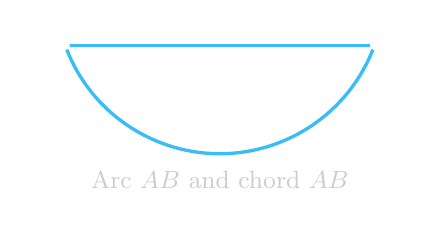
\begin{tikzpicture}[scale=0.95]
  \def\r{2.2}
  \coordinate (A) at ({\r*cos(200)},{\r*sin(200)});
  \coordinate (B) at ({\r*cos(340)},{\r*sin(340)});
  \draw[new] (A) arc (200:340:\r);
  \draw[new] (A)--(B);
  \node[dot] at (A) {}; \node[lab] at ($(A)+(-0.25,0)$) {$A$};
  \node[dot] at (B) {}; \node[lab] at ($(B)+(0.25,0)$) {$B$};
  \node[labm] at (0,-2.55) {Arc $AB$ and chord $AB$};
\end{tikzpicture}
\end{StepDiagram}

\Step{2} Construct the perpendicular bisector of $AB$ (use equal arcs from $A$ and $B$ to meet at $X$ and $Y$).
\begin{StepDiagram}
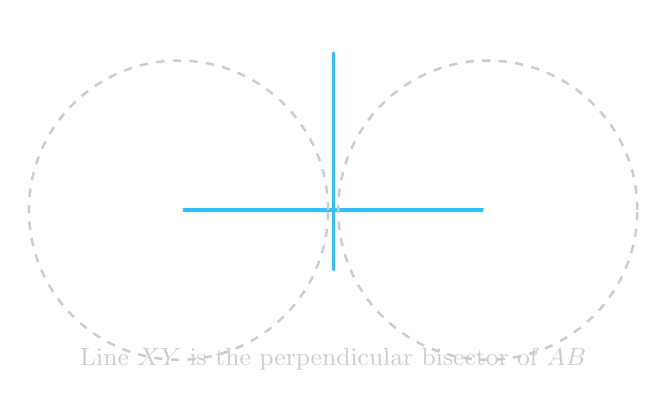
\begin{tikzpicture}[scale=0.95]
  \def\r{2.2}
  \coordinate (A) at ({\r*cos(200)},{\r*sin(200)});
  \coordinate (B) at ({\r*cos(340)},{\r*sin(340)});
  \coordinate (X) at (0,1.35);
  \coordinate (Y) at (0,-1.55);

  \draw[base] (A) arc (200:340:\r);
  \draw[new] (A)--(B);

  % construction arcs (illustrative)
  \draw[help] (A) circle (2.0);
  \draw[help] (B) circle (2.0);

  \node[dot] at (A) {}; \node[lab] at ($(A)+(-0.25,0)$) {$A$};
  \node[dot] at (B) {}; \node[lab] at ($(B)+(0.25,0)$) {$B$};
  \node[dot] at (X) {}; \node[lab] at ($(X)+(0.18,0.1)$) {$X$};
  \node[dot] at (Y) {}; \node[lab] at ($(Y)+(0.18,-0.05)$) {$Y$};

  \draw[new] (X)--(Y);
  \node[labm] at (0,-2.75) {Line $XY$ is the perpendicular bisector of $AB$};
\end{tikzpicture}
\end{StepDiagram}

\Step{3} Let the perpendicular bisector meet the arc at $M$. Then $\widehat{AM}=\widehat{MB}$.
\begin{StepDiagram}
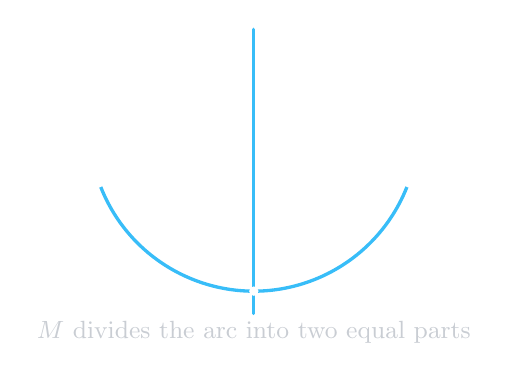
\begin{tikzpicture}[scale=0.95]
  \def\r{2.2}
  \coordinate (A) at ({\r*cos(200)},{\r*sin(200)});
  \coordinate (B) at ({\r*cos(340)},{\r*sin(340)});
  \coordinate (M) at ({\r*cos(270)},{\r*sin(270)});
  \draw[new] (A) arc (200:340:\r);
  \draw[base] (A)--(B);
  \draw[new] (0,-2.5)--(0,1.3);
  \node[dot] at (A) {}; \node[lab] at ($(A)+(-0.25,0)$) {$A$};
  \node[dot] at (B) {}; \node[lab] at ($(B)+(0.25,0)$) {$B$};
  \node[dot] at (M) {}; \node[lab] at ($(M)+(0,-0.30)$) {$M$};
  \node[labm] at (0,-2.75) {$M$ divides the arc into two equal parts};
\end{tikzpicture}
\end{StepDiagram}

\end{QAPair}

% ============================================================
% Q2
\begin{QAPair}{Question 2}
\textcolor{gold}{\bfseries Question:} Draw an arc of any length. Draw a tangent \emph{without using centre}, through point $A$,
when $A$ is (i) in the middle of arc, (ii) at the right end of the arc.
\tcblower
\textcolor{green}{\bfseries Construction (Alternate Segment Theorem):}\par

\Step{1} On the arc, mark point $A$ and choose two other points $B$ and $C$ on the arc (anywhere convenient).
\begin{StepDiagram}
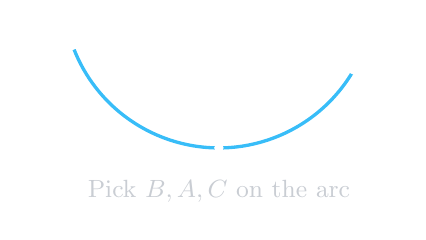
\begin{tikzpicture}[scale=0.92]
  \def\r{2.15}
  \coordinate (B) at ({\r*cos(200)},{\r*sin(200)});
  \coordinate (A) at ({\r*cos(270)},{\r*sin(270)});
  \coordinate (C) at ({\r*cos(330)},{\r*sin(330)});
  \draw[new] (B) arc (200:330:\r);
  \node[dot,label={[lab]below:$A$}] at (A) {};
  \node[dot,label={[lab]left:$B$}] at (B) {};
  \node[dot,label={[lab]right:$C$}] at (C) {};
  \node[labm] at (0,-2.75) {Pick $B,A,C$ on the arc};
\end{tikzpicture}
\end{StepDiagram}

\Step{2} Join $AB$, $AC$ and $BC$ to form $\angle ACB$ on the circle.
\begin{StepDiagram}
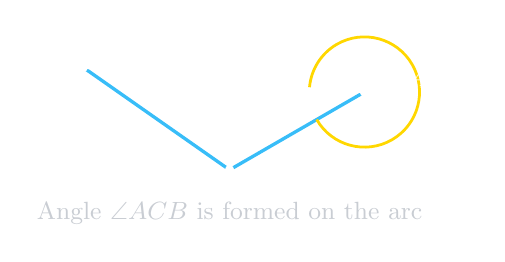
\begin{tikzpicture}[scale=0.92]
  \def\r{2.15}
  \coordinate (B) at ({\r*cos(200)},{\r*sin(200)});
  \coordinate (A) at ({\r*cos(270)},{\r*sin(270)});
  \coordinate (C) at ({\r*cos(330)},{\r*sin(330)});
  \draw[base] (B) arc (200:330:\r);
  \draw[new] (A)--(B);
  \draw[new] (A)--(C);
  \draw[base] (B)--(C);
  \node[dot,label={[lab]below:$A$}] at (A) {};
  \node[dot,label={[lab]left:$B$}] at (B) {};
  \node[dot,label={[lab]right:$C$}] at (C) {};
  \pic[ang,"$\angle ACB$",lab,angle radius=7mm,angle eccentricity=1.2] {angle=A--C--B};
  \node[labm] at (0,-2.75) {Angle $\angle ACB$ is formed on the arc};
\end{tikzpicture}
\end{StepDiagram}

\Step{3} At $A$, draw a line making an angle with chord $AB$ equal to $\angle ACB$, but outside the arc. This line is the tangent at $A$.
\begin{StepDiagram}
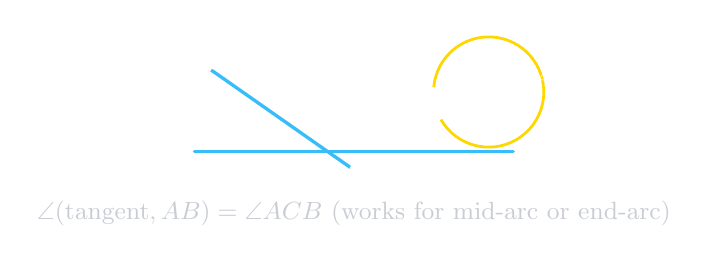
\begin{tikzpicture}[scale=0.92]
  \def\r{2.15}
  \coordinate (B) at ({\r*cos(200)},{\r*sin(200)});
  \coordinate (A) at ({\r*cos(270)},{\r*sin(270)});
  \coordinate (C) at ({\r*cos(330)},{\r*sin(330)});
  \coordinate (T1) at ($(A)+(-2.2,0.25)$);
  \coordinate (T2) at ($(A)+( 2.2,0.25)$);

  \draw[base] (B) arc (200:330:\r);
  \draw[new] (A)--(B);
  \draw[base] (B)--(C);
  \draw[base] (A)--(C);
  \draw[new] (T1)--(T2); % tangent

  \node[dot,label={[lab]below:$A$}] at (A) {};
  \node[dot,label={[lab]left:$B$}] at (B) {};
  \node[dot,label={[lab]right:$C$}] at (C) {};
  \pic[ang,"$\angle ACB$",lab,angle radius=7mm,angle eccentricity=1.2] {angle=A--C--B};
  \node[labm] at (0,-2.75) {$\angle(\text{tangent},AB)=\angle ACB$ (works for mid-arc or end-arc)};
\end{tikzpicture}
\end{StepDiagram}

\end{QAPair}

% ============================================================
% Q3
\begin{QAPair}{Question 3}
\textcolor{gold}{\bfseries Question:} Draw an arc $ABC$. Take a point $X$ outside the arc and draw a tangent from $X$ to the arc without using centre of the arc.
\tcblower
\textcolor{green}{\bfseries Construction:}\par

\Step{1} Draw the arc (part of a circle) and mark points $A,B,C$ on it. Take an external point $X$.
\begin{StepDiagram}
\begin{tikzpicture}[scale=0.9]
  \def\r{2.0}
  \coordinate (O) at (0,0); % hidden centre (not used yet)
  \coordinate (A) at ({\r*cos(150)},{\r*sin(150)});
  \coordinate (B) at ({\r*cos(230)},{\r*sin(230)});
  \coordinate (C) at ({\r*cos(320)},{\r*sin(320)});
  \coordinate (X) at (3.4,1.5);
  \draw[new] (A) arc (150:320:\r);
  \node[dot,label={[lab]left:$A$}] at (A) {};
  \node[dot,label={[lab]below left:$B$}] at (B) {};
  \node[dot,label={[lab]right:$C$}] at (C) {};
  \node[dot,label={[lab]right:$X$}] at (X) {};
  \node[labm] at (0,-2.55) {Given arc $ABC$ and external point $X$};
\end{tikzpicture}
\end{StepDiagram}

\Step{2} Join chords $AB$ and $BC$.
\begin{StepDiagram}
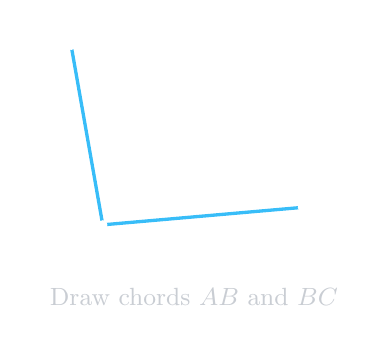
\begin{tikzpicture}[scale=0.9]
  \def\r{2.0}
  \coordinate (A) at ({\r*cos(150)},{\r*sin(150)});
  \coordinate (B) at ({\r*cos(230)},{\r*sin(230)});
  \coordinate (C) at ({\r*cos(320)},{\r*sin(320)});
  \draw[base] (A) arc (150:320:\r);
  \draw[new] (A)--(B);
  \draw[new] (B)--(C);
  \node[dot,label={[lab]left:$A$}] at (A) {};
  \node[dot,label={[lab]below left:$B$}] at (B) {};
  \node[dot,label={[lab]right:$C$}] at (C) {};
  \node[labm] at (0,-2.55) {Draw chords $AB$ and $BC$};
\end{tikzpicture}
\end{StepDiagram}

\Step{3} Construct perpendicular bisectors of $AB$ and $BC$. Their intersection gives the centre $O$ of the circle of the arc.
\begin{StepDiagram}
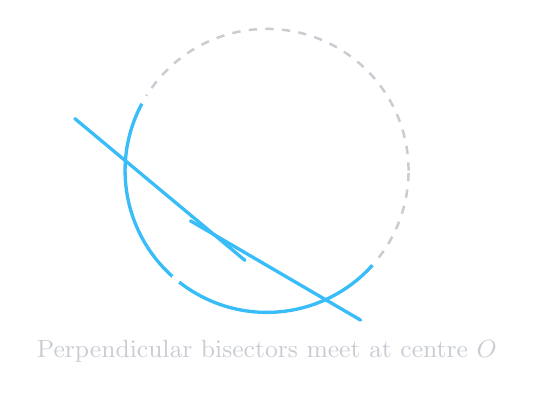
\begin{tikzpicture}[scale=0.9]
  \def\r{2.0}
  \coordinate (O) at (0,0);
  \coordinate (A) at ({\r*cos(150)},{\r*sin(150)});
  \coordinate (B) at ({\r*cos(230)},{\r*sin(230)});
  \coordinate (C) at ({\r*cos(320)},{\r*sin(320)});
  \coordinate (Mab) at ($(A)!0.5!(B)$);
  \coordinate (Mbc) at ($(B)!0.5!(C)$);

  \draw[help] (O) circle (\r);
  \draw[new] (A) arc (150:320:\r);
  \draw[base] (A)--(B);
  \draw[base] (B)--(C);

  \draw[new] ($(Mab)+(-1.2,1.0)$)--($(Mab)+(1.2,-1.0)$);
  \draw[new] ($(Mbc)+(-1.2,0.7)$)--($(Mbc)+(1.2,-0.7)$);

  \node[dot,label={[lab]below:$O$}] at (O) {};
  \node[dot,label={[lab]left:$A$}] at (A) {};
  \node[dot,label={[lab]below left:$B$}] at (B) {};
  \node[dot,label={[lab]right:$C$}] at (C) {};
  \node[labm] at (0,-2.55) {Perpendicular bisectors meet at centre $O$};
\end{tikzpicture}
\end{StepDiagram}

\Step{4} Join $OX$. Draw the circle with diameter $OX$; it meets the circle at $T_1,T_2$. Join $XT_1$ (or $XT_2$): required tangent(s).
\begin{StepDiagram}
\begin{tikzpicture}[scale=0.9]
  \def\r{2.0}
  \coordinate (O) at (0,0);
  \coordinate (X) at (3.4,1.5);
  \coordinate (M) at ($(O)!0.5!(X)$);

  \draw[help] (O) circle (\r);           % original (full) circle
  \draw[base] (O)--(X);                 % OX
  \draw[help] (M) circle ({veclen((X)-(M))}); % diameter circle

  % illustrative tangency points on original circle
  \coordinate (T1) at ({\r*cos(20)},{\r*sin(20)});
  \coordinate (T2) at ({\r*cos(80)},{\r*sin(80)});
  \draw[new] (X)--(T1);
  \draw[new] (X)--(T2);

  \node[dot,label={[lab]below:$O$}] at (O) {};
  \node[dot,label={[lab]right:$X$}] at (X) {};
  \node[dot,label={[lab]right:$T_1$}] at (T1) {};
  \node[dot,label={[lab]left:$T_2$}] at (T2) {};

  \node[labm] at (0,-2.55) {Circle on diameter $OX$ gives tangency points};
\end{tikzpicture}
\end{StepDiagram}

\end{QAPair}

% ============================================================
% Q4
\begin{QAPair}{Question 4}
\textcolor{gold}{\bfseries Question:} Construct a circle of radius $4$ cm. Mark a point $P$ on the circumference and draw a tangent passing through $P$.
\tcblower
\textcolor{green}{\bfseries Construction:}\par

\Step{1} Draw a circle with centre $O$ and radius $4$ cm.
\begin{StepDiagram}
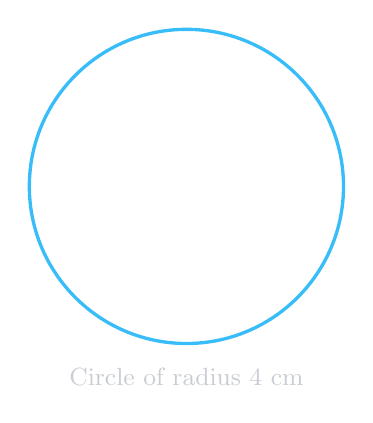
\begin{tikzpicture}[scale=0.95]
  \def\r{2.1}
  \coordinate (O) at (0,0);
  \draw[new] (O) circle (\r);
  \node[dot,label={[lab]below:$O$}] at (O) {};
  \node[labm] at (0,-2.55) {Circle of radius $4$ cm};
\end{tikzpicture}
\end{StepDiagram}

\Step{2} Mark point $P$ on the circle and join $OP$.
\begin{StepDiagram}
\begin{tikzpicture}[scale=0.95]
  \def\r{2.1}
  \coordinate (O) at (0,0);
  \coordinate (P) at ({\r*cos(40)},{\r*sin(40)});
  \draw[base] (O) circle (\r);
  \node[dot,label={[lab]below:$O$}] at (O) {};
  \node[dot,label={[lab]right:$P$}] at (P) {};
  \draw[new] (O)--(P);
  \node[labm] at (0,-2.55) {Draw radius $OP$};
\end{tikzpicture}
\end{StepDiagram}

\Step{3} Draw a line at $P$ perpendicular to $OP$; it is the tangent.
\begin{StepDiagram}
\begin{tikzpicture}[scale=0.95]
  \def\r{2.1}
  \coordinate (O) at (0,0);
  \coordinate (P) at ({\r*cos(40)},{\r*sin(40)});
  \coordinate (T1) at ($(P)+({-1.9*sin(40)},{1.9*cos(40)})$);
  \coordinate (T2) at ($(P)+({ 1.9*sin(40)},{-1.9*cos(40)})$);
  \draw[base] (O) circle (\r);
  \node[dot,label={[lab]below:$O$}] at (O) {};
  \node[dot,label={[lab]right:$P$}] at (P) {};
  \draw[new] (O)--(P);
  \draw[new] (T1)--(T2);
  \draw[base] ($(P)+(0.16,0)$) -- ($(P)+(0.16,-0.16)$) -- ($(P)+(0,-0.16)$);
  \node[labm] at (0,-2.55) {$OP\perp$ tangent};
\end{tikzpicture}
\end{StepDiagram}

\end{QAPair}

% ============================================================
% Q5
\begin{QAPair}{Question 5}
\textcolor{gold}{\bfseries Question:} Construct a circle of radius $3$ cm. Draw two tangents from a point $A$, $5.8$ cm away from the centre of circle.
\tcblower
\textcolor{green}{\bfseries Construction:}\par

\Step{1} Draw the circle with centre $O$ and radius $3$ cm.
\begin{StepDiagram}
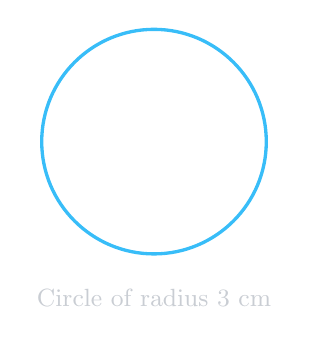
\begin{tikzpicture}[scale=0.92]
  \def\r{1.55}
  \coordinate (O) at (0,0);
  \draw[new] (O) circle (\r);
  \node[dot,label={[lab]below:$O$}] at (O) {};
  \node[labm] at (0,-2.15) {Circle of radius $3$ cm};
\end{tikzpicture}
\end{StepDiagram}

\Step{2} Mark point $A$ such that $OA=5.8$ cm and join $OA$.
\begin{StepDiagram}
\begin{tikzpicture}[scale=0.92]
  \def\r{1.55}
  \coordinate (O) at (0,0);
  \coordinate (A) at (3.5,0.8);
  \draw[base] (O) circle (\r);
  \node[dot,label={[lab]below:$O$}] at (O) {};
  \node[dot,label={[lab]right:$A$}] at (A) {};
  \draw[new] (O)--(A);
  \node[labm] at (0,-2.15) {Draw $OA$ (given distance)};
\end{tikzpicture}
\end{StepDiagram}

\Step{3} Draw a circle with diameter $OA$ (centre at midpoint of $OA$).
\begin{StepDiagram}
\begin{tikzpicture}[scale=0.92]
  \def\r{1.55}
  \coordinate (O) at (0,0);
  \coordinate (A) at (3.5,0.8);
  \coordinate (M) at ($(O)!0.5!(A)$);
  \draw[base] (O) circle (\r);
  \draw[new] (O)--(A);
  \draw[help] (M) circle ({veclen((A)-(M))});
  \node[dot,label={[lab]below:$O$}] at (O) {};
  \node[dot,label={[lab]right:$A$}] at (A) {};
  \node[dot,label={[lab]above:$M$}] at (M) {};
  \node[labm] at (0,-2.15) {Auxiliary circle on diameter $OA$};
\end{tikzpicture}
\end{StepDiagram}

\Step{4} Let the auxiliary circle cut the given circle at $T_1,T_2$. Join $AT_1$ and $AT_2$; these are the tangents.
\begin{StepDiagram}
\begin{tikzpicture}[scale=0.92]
  \def\r{1.55}
  \coordinate (O) at (0,0);
  \coordinate (A) at (3.5,0.8);
  \coordinate (M) at ($(O)!0.5!(A)$);
  \draw[base] (O) circle (\r);
  \draw[base] (O)--(A);
  \draw[help] (M) circle ({veclen((A)-(M))});

  \coordinate (T1) at ({\r*cos(20)},{\r*sin(20)});
  \coordinate (T2) at ({\r*cos(90)},{\r*sin(90)});
  \draw[new] (A)--(T1);
  \draw[new] (A)--(T2);

  \node[dot,label={[lab]below:$O$}] at (O) {};
  \node[dot,label={[lab]right:$A$}] at (A) {};
  \node[dot,label={[lab]right:$T_1$}] at (T1) {};
  \node[dot,label={[lab]above:$T_2$}] at (T2) {};

  \node[labm] at (0,-2.15) {Tangents from $A$ touch at $T_1,T_2$};
\end{tikzpicture}
\end{StepDiagram}

\end{QAPair}

% ============================================================
% Q6
\begin{QAPair}{Question 6}
\textcolor{gold}{\bfseries Question:} Construct a circle of radius $2.5$ cm. Draw two tangents making an angle of: (i) $45^\circ$ (ii) $90^\circ$ with each other.
\tcblower
\textcolor{green}{\bfseries Construction:}\par

\Step{1} Draw the circle with centre $O$ and radius $2.5$ cm.
\begin{StepDiagram}
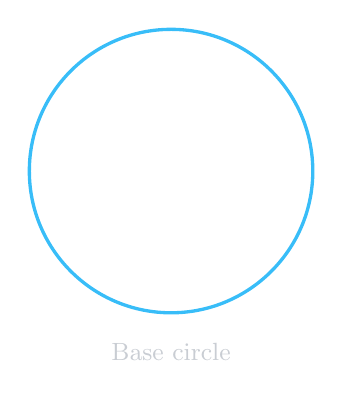
\begin{tikzpicture}[scale=0.9]
  \def\r{2.0}
  \coordinate (O) at (0,0);
  \draw[new] (O) circle (\r);
  \node[dot,label={[lab]below:$O$}] at (O) {};
  \node[labm] at (0,-2.55) {Base circle};
\end{tikzpicture}
\end{StepDiagram}

\Step{2} Use $\angle(\text{tangents})=180^\circ-\angle AOB$.  
For $45^\circ$, construct $\angle AOB=135^\circ$; for $90^\circ$, construct $\angle AOB=90^\circ$.
\EqDiagram{$\angle APB=\theta \Rightarrow \angle AOB=180^\circ-\theta$:\quad
(i)\ \theta=45^\circ\Rightarrow\angle AOB=135^\circ,\quad
(ii)\ \theta=90^\circ\Rightarrow\angle AOB=90^\circ.$}

\Step{3} Mark points $A,B$ on the circle so that $\angle AOB$ equals the required value.
\begin{StepDiagram}
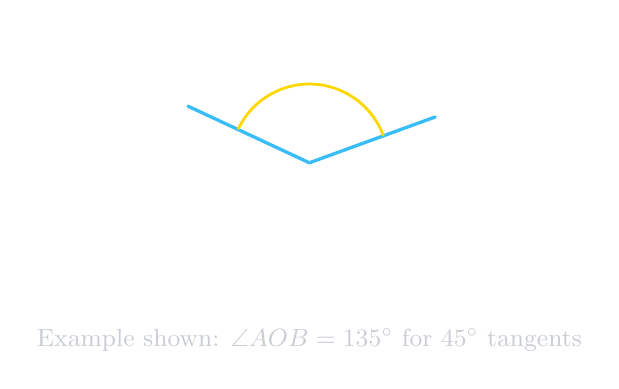
\begin{tikzpicture}[scale=0.85]
  \def\r{2.0}
  \coordinate (O) at (0,0);
  \coordinate (A) at ({\r*cos(20)},{\r*sin(20)});
  \coordinate (B) at ({\r*cos(155)},{\r*sin(155)});
  \draw[base] (O) circle (\r);
  \node[dot,label={[lab]below:$O$}] at (O) {};
  \node[dot,label={[lab]right:$A$}] at (A) {};
  \node[dot,label={[lab]left:$B$}] at (B) {};
  \draw[new] (O)--(A);
  \draw[new] (O)--(B);
  \pic[ang,"$135^\circ$",lab,angle radius=10mm,angle eccentricity=1.15] {angle=A--O--B};
  \node[labm] at (0,-2.65) {Example shown: $\angle AOB=135^\circ$ for $45^\circ$ tangents};
\end{tikzpicture}
\end{StepDiagram}

\Step{4} Draw tangents at $A$ and $B$ (perpendicular to $OA$ and $OB$). Their intersection gives the required angle.
\begin{StepDiagram}
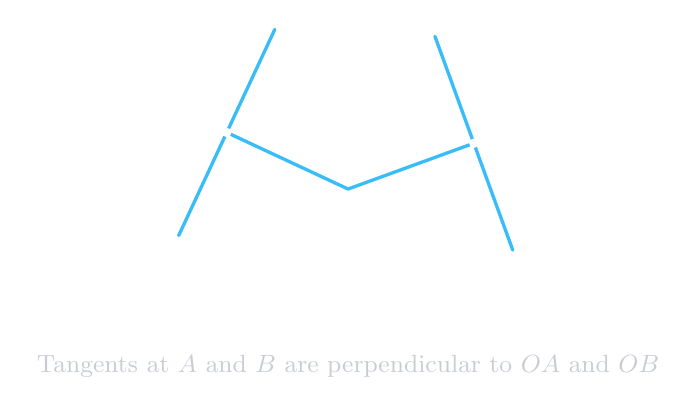
\begin{tikzpicture}[scale=0.85]
  \def\r{2.0}
  \coordinate (O) at (0,0);
  \coordinate (A) at ({\r*cos(20)},{\r*sin(20)});
  \coordinate (B) at ({\r*cos(155)},{\r*sin(155)});

  \coordinate (TA1) at ($(A)+({-1.7*sin(20)},{1.7*cos(20)})$);
  \coordinate (TA2) at ($(A)+({ 1.7*sin(20)},{-1.7*cos(20)})$);
  \coordinate (TB1) at ($(B)+({-1.7*sin(155)},{1.7*cos(155)})$);
  \coordinate (TB2) at ($(B)+({ 1.7*sin(155)},{-1.7*cos(155)})$);

  \draw[base] (O) circle (\r);
  \node[dot,label={[lab]below:$O$}] at (O) {};
  \draw[new] (O)--(A);
  \draw[new] (O)--(B);
  \draw[new] (TA1)--(TA2);
  \draw[new] (TB1)--(TB2);
  \node[dot,label={[lab]right:$A$}] at (A) {};
  \node[dot,label={[lab]left:$B$}] at (B) {};

  \node[labm] at (0,-2.65) {Tangents at $A$ and $B$ are perpendicular to $OA$ and $OB$};
\end{tikzpicture}
\end{StepDiagram}

\end{QAPair}

% ============================================================
% Q7
\begin{QAPair}{Question 7}
\textcolor{gold}{\bfseries Question:} Construct two equal circles each of radius $3$ cm. Centres are $6$ cm apart. Draw their:
(i) direct common tangents, (ii) transverse common tangents.
\tcblower
\textcolor{green}{\bfseries Construction:}\par

\Step{1} Draw $O_1O_2=6$ cm and draw two circles of radius $3$ cm.
\begin{StepDiagram}
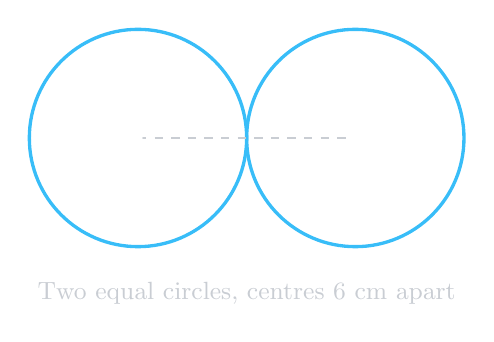
\begin{tikzpicture}[scale=0.92]
  \def\R{1.5}
  \def\d{3.0}
  \coordinate (O1) at (0,0);
  \coordinate (O2) at (\d,0);
  \draw[new] (O1) circle (\R);
  \draw[new] (O2) circle (\R);
  \draw[help] (O1)--(O2);
  \node[dot,label={[lab]below:$O_1$}] at (O1) {};
  \node[dot,label={[lab]below:$O_2$}] at (O2) {};
  \node[labm] at (1.5,-2.15) {Two equal circles, centres $6$ cm apart};
\end{tikzpicture}
\end{StepDiagram}

\Step{2} Draw the two \textbf{direct} common tangents (top and bottom): lines parallel to $O_1O_2$ touching both circles.
\begin{StepDiagram}
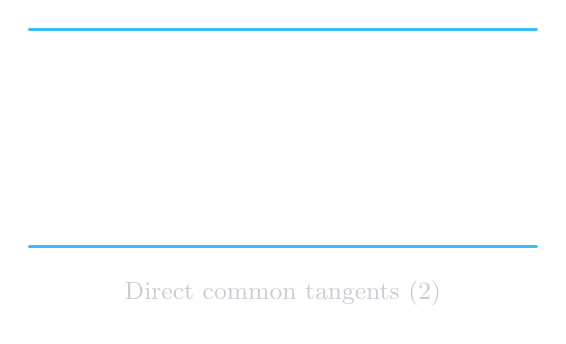
\begin{tikzpicture}[scale=0.92]
  \def\R{1.5}
  \def\d{3.0}
  \coordinate (O1) at (0,0);
  \coordinate (O2) at (\d,0);
  \draw[base] (O1) circle (\R);
  \draw[base] (O2) circle (\R);
  \draw[new] (-2, \R) -- (5, \R);
  \draw[new] (-2,-\R) -- (5,-\R);
  \node[dot,label={[lab]below:$O_1$}] at (O1) {};
  \node[dot,label={[lab]below:$O_2$}] at (O2) {};
  \node[labm] at (1.5,-2.15) {Direct common tangents (2)};
\end{tikzpicture}
\end{StepDiagram}

\Step{3} Since circles touch, the \textbf{transverse} common tangent is at the contact point $T$ and is perpendicular to $O_1O_2$.
\begin{StepDiagram}
\begin{tikzpicture}[scale=0.92]
  \def\R{1.5}
  \def\d{3.0}
  \coordinate (O1) at (0,0);
  \coordinate (O2) at (\d,0);
  \coordinate (T) at (\R,0);
  \draw[base] (O1) circle (\R);
  \draw[base] (O2) circle (\R);
  \draw[help] (O1)--(O2);
  \draw[new] (\R,-2.2) -- (\R,2.2);
  \node[dot,label={[lab]below:$O_1$}] at (O1) {};
  \node[dot,label={[lab]below:$O_2$}] at (O2) {};
  \node[dot,label={[lab]below:$T$}] at (T) {};
  \node[labm] at (1.5,-2.15) {Transverse tangent at contact point};
\end{tikzpicture}
\end{StepDiagram}

\end{QAPair}

% ============================================================
% Q8
\begin{QAPair}{Question 8}
\textcolor{gold}{\bfseries Question:} Construct two circles of radii $2$ cm and $3.5$ cm, distance between centres $6.4$ cm.
Draw (i) direct common tangents (ii) transverse common tangents.
\tcblower
\textcolor{green}{\bfseries Construction (auxiliary-circle method):}\par

Let bigger radius $R=3.5$ and smaller radius $r=2$.

\Step{1} Draw $O_1O_2=6.4$ cm and draw the circles $(O_1,R)$ and $(O_2,r)$.
\begin{StepDiagram}
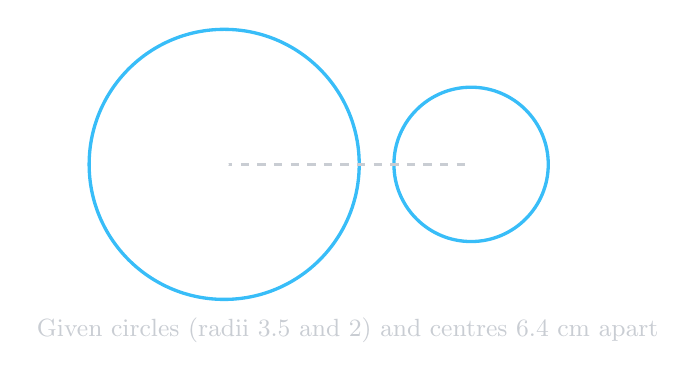
\begin{tikzpicture}[scale=0.98]
  \pgfmathsetmacro{\R}{1.75} % scaled by 0.5
  \pgfmathsetmacro{\r}{1.00}
  \pgfmathsetmacro{\d}{3.20}
  \coordinate (O1) at (0,0);
  \coordinate (O2) at (\d,0);
  \draw[new] (O1) circle (\R);
  \draw[new] (O2) circle (\r);
  \draw[help] (O1)--(O2);
  \node[dot,label={[lab]below:$O_1$}] at (O1) {};
  \node[dot,label={[lab]below:$O_2$}] at (O2) {};
  \node[labm] at (1.6,-2.15) {Given circles (radii $3.5$ and $2$) and centres $6.4$ cm apart};
\end{tikzpicture}
\end{StepDiagram}

\Step{2} For \textbf{direct} tangents, draw auxiliary circle with centre $O_1$ and radius $(R-r)=1.5$ cm.
\begin{StepDiagram}
\begin{tikzpicture}[scale=0.98]
  \pgfmathsetmacro{\R}{1.75}
  \pgfmathsetmacro{\r}{1.00}
  \pgfmathsetmacro{\d}{3.20}
  \pgfmathsetmacro{\aux}{0.75} % (R-r)=1.5 scaled by 0.5
  \coordinate (O1) at (0,0);
  \coordinate (O2) at (\d,0);

  \draw[base] (O1) circle (\R);
  \draw[base] (O2) circle (\r);
  \draw[new]  (O1) circle (\aux);
  \node[dot,label={[lab]below:$O_1$}] at (O1) {};
  \node[dot,label={[lab]below:$O_2$}] at (O2) {};
  \node[labm] at (1.6,-2.15) {Auxiliary circle radius $R-r$ (for direct tangents)};
\end{tikzpicture}
\end{StepDiagram}

\Step{3} From $O_2$, draw two tangents to the auxiliary circle.
\begin{StepDiagram}
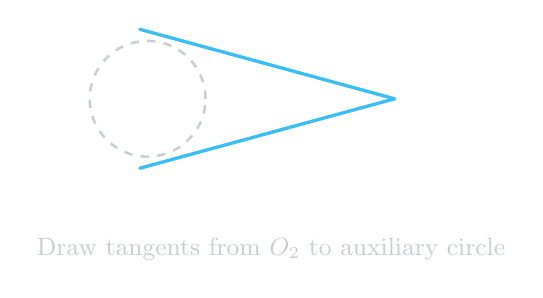
\begin{tikzpicture}[scale=0.98]
  \pgfmathsetmacro{\R}{1.75}
  \pgfmathsetmacro{\r}{1.00}
  \pgfmathsetmacro{\d}{3.20}
  \pgfmathsetmacro{\aux}{0.75}
  \coordinate (O1) at (0,0);
  \coordinate (O2) at (\d,0);

  \draw[help] (O1) circle (\aux);
  \node[dot,label={[lab]below:$O_1$}] at (O1) {};
  \node[dot,label={[lab]below:$O_2$}] at (O2) {};

  % just illustrative tangent lines from O2 to aux circle
  \draw[new] (O2)--(-0.10, 0.90);
  \draw[new] (O2)--(-0.10,-0.90);

  \node[labm] at (1.6,-1.95) {Draw tangents from $O_2$ to auxiliary circle};
\end{tikzpicture}
\end{StepDiagram}

\Step{4} Draw lines parallel to those tangents that touch the smaller circle; these are the \textbf{direct} common tangents.
\begin{StepDiagram}
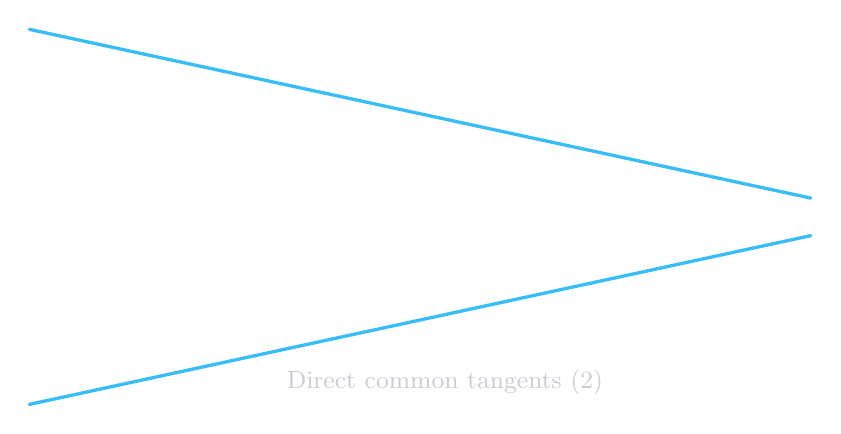
\begin{tikzpicture}[scale=0.98]
  \pgfmathsetmacro{\R}{1.75}
  \pgfmathsetmacro{\r}{1.00}
  \pgfmathsetmacro{\d}{3.20}
  \coordinate (O1) at (0,0);
  \coordinate (O2) at (\d,0);

  \draw[base] (O1) circle (\R);
  \draw[base] (O2) circle (\r);

  % direct tangents (computed)
  \pgfmathsetmacro{\nxE}{(\R-\r)/\d}
  \pgfmathsetmacro{\nyE}{sqrt(1-\nxE*\nxE)}
  \coordinate (P1t) at ({- \R*\nxE},{- \R*\nyE});
  \coordinate (P2t) at ({\d- \r*\nxE},{- \r*\nyE});
  \coordinate (P1b) at ({- \R*\nxE},{+ \R*\nyE});
  \coordinate (P2b) at ({\d- \r*\nxE},{+ \r*\nyE});
  \draw[new] ($(P1t)!-1.0!(P2t)$) -- ($(P1t)!2.0!(P2t)$);
  \draw[new] ($(P1b)!-1.0!(P2b)$) -- ($(P1b)!2.0!(P2b)$);

  \node[dot,label={[lab]below:$O_1$}] at (O1) {};
  \node[dot,label={[lab]below:$O_2$}] at (O2) {};
  \node[labm] at (1.6,-2.15) {Direct common tangents (2)};
\end{tikzpicture}
\end{StepDiagram}

\Step{5} For \textbf{transverse} tangents, draw auxiliary circle with centre $O_1$ and radius $(R+r)=5.5$ cm.
\begin{StepDiagram}
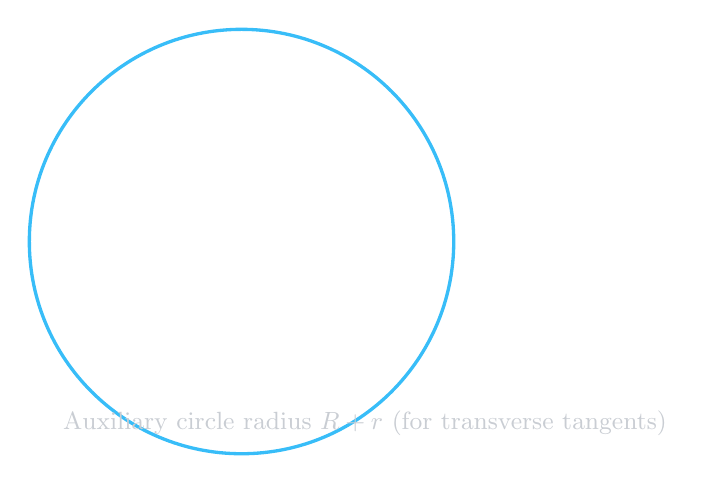
\begin{tikzpicture}[scale=0.98]
  \pgfmathsetmacro{\R}{1.75}
  \pgfmathsetmacro{\r}{1.00}
  \pgfmathsetmacro{\d}{3.20}
  \pgfmathsetmacro{\aux}{2.75} % (R+r)=5.5 scaled by 0.5
  \coordinate (O1) at (0,0);
  \coordinate (O2) at (\d,0);
  \draw[base] (O1) circle (\R);
  \draw[base] (O2) circle (\r);
  \draw[new]  (O1) circle (\aux);
  \node[dot,label={[lab]below:$O_1$}] at (O1) {};
  \node[dot,label={[lab]below:$O_2$}] at (O2) {};
  \node[labm] at (1.6,-2.35) {Auxiliary circle radius $R+r$ (for transverse tangents)};
\end{tikzpicture}
\end{StepDiagram}

\Step{6} From $O_2$, draw two tangents to this $(R+r)$ auxiliary circle.
\begin{StepDiagram}
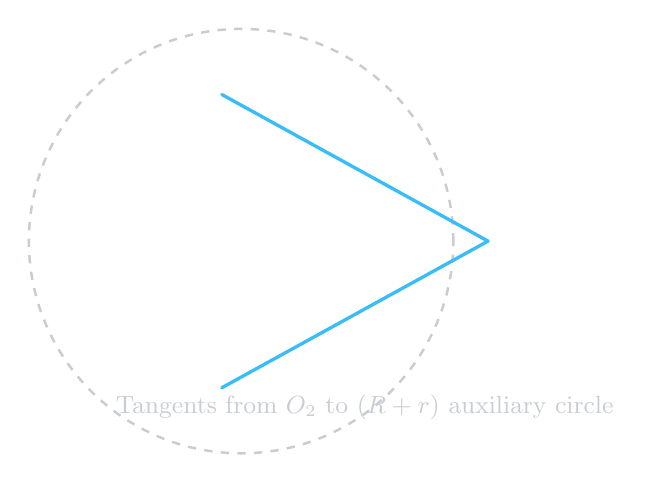
\begin{tikzpicture}[scale=0.98]
  \pgfmathsetmacro{\aux}{2.75}
  \coordinate (O1) at (0,0);
  \coordinate (O2) at (3.20,0);
  \draw[help] (O1) circle (\aux);
  \node[dot,label={[lab]below:$O_1$}] at (O1) {};
  \node[dot,label={[lab]below:$O_2$}] at (O2) {};
  \draw[new] (O2)--(-0.25, 1.90);
  \draw[new] (O2)--(-0.25,-1.90);
  \node[labm] at (1.6,-2.15) {Tangents from $O_2$ to $(R+r)$ auxiliary circle};
\end{tikzpicture}
\end{StepDiagram}

\Step{7} Draw parallels touching the smaller circle on the opposite side; these are the \textbf{transverse} common tangents.
\begin{StepDiagram}
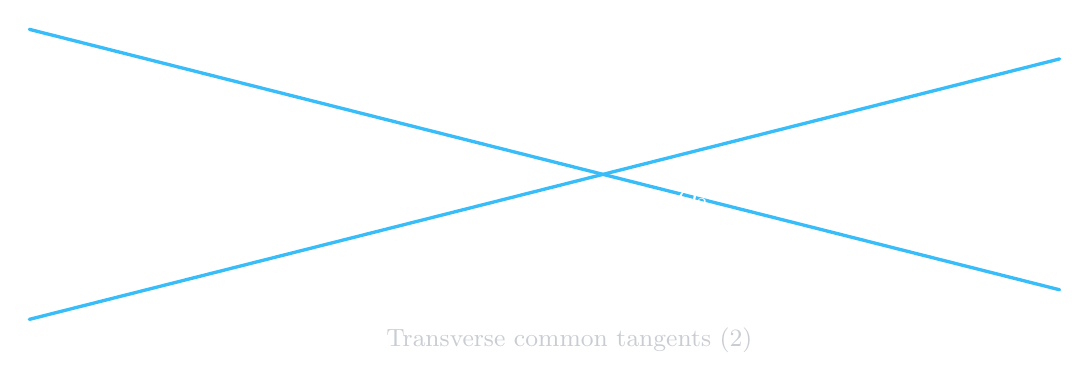
\begin{tikzpicture}[scale=0.98]
  \pgfmathsetmacro{\R}{1.75}
  \pgfmathsetmacro{\r}{1.00}
  \pgfmathsetmacro{\d}{3.20}
  \coordinate (O1) at (0,0);
  \coordinate (O2) at (\d,0);

  \draw[base] (O1) circle (\R);
  \draw[base] (O2) circle (\r);

  % transverse tangents (computed)
  \pgfmathsetmacro{\nxI}{(\R+\r)/\d}
  \pgfmathsetmacro{\nyI}{sqrt(1-\nxI*\nxI)}
  \coordinate (Q1t) at ({- \R*\nxI},{- \R*\nyI});
  \coordinate (Q2t) at ({\d+ \r*\nxI},{+ \r*\nyI});
  \coordinate (Q1b) at ({- \R*\nxI},{+ \R*\nyI});
  \coordinate (Q2b) at ({\d+ \r*\nxI},{- \r*\nyI});
  \draw[new] ($(Q1t)!-0.7!(Q2t)$) -- ($(Q1t)!1.7!(Q2t)$);
  \draw[new] ($(Q1b)!-0.7!(Q2b)$) -- ($(Q1b)!1.7!(Q2b)$);

  \node[dot,label={[lab]below:$O_1$}] at (O1) {};
  \node[dot,label={[lab]below:$O_2$}] at (O2) {};
  \node[labm] at (1.6,-2.15) {Transverse common tangents (2)};
\end{tikzpicture}
\end{StepDiagram}

\end{QAPair}

% ============================================================
% Q9
\begin{QAPair}{Question 9}
\textcolor{gold}{\bfseries Question:} Construct two touching circles of radii $2.6$ cm and $3.6$ cm. Draw:
(i) a common tangent through the point of contact,
(ii) a common tangent not through the point of contact,
(iii) two common tangents.
\tcblower
\textcolor{green}{\bfseries Construction:}\par

\Step{1} Draw $O_1O_2=2.6+3.6=6.2$ cm and draw both circles.
\begin{StepDiagram}
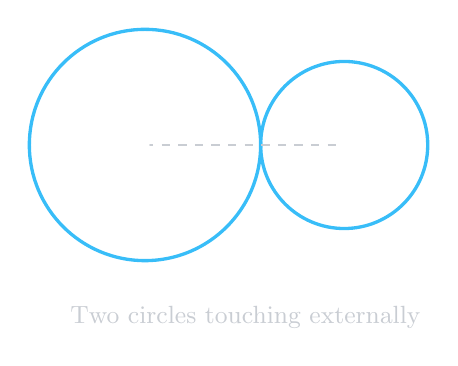
\begin{tikzpicture}[scale=1.02]
  \pgfmathsetmacro{\R}{1.44} % 3.6 scaled by 0.4
  \pgfmathsetmacro{\r}{1.04} % 2.6 scaled by 0.4
  \pgfmathsetmacro{\d}{2.48} % 6.2 scaled by 0.4
  \coordinate (O1) at (0,0);
  \coordinate (O2) at (\d,0);
  \draw[new] (O1) circle (\R);
  \draw[new] (O2) circle (\r);
  \draw[help] (O1)--(O2);
  \node[dot,label={[lab]below:$O_1$}] at (O1) {};
  \node[dot,label={[lab]below:$O_2$}] at (O2) {};
  \node[labm] at (1.25,-2.15) {Two circles touching externally};
\end{tikzpicture}
\end{StepDiagram}

\Step{2} Mark the point of contact $T$ on $O_1O_2$ and draw tangent at $T$ perpendicular to $O_1O_2$.
\begin{StepDiagram}
\begin{tikzpicture}[scale=1.02]
  \pgfmathsetmacro{\R}{1.44}
  \pgfmathsetmacro{\r}{1.04}
  \pgfmathsetmacro{\d}{2.48}
  \coordinate (O1) at (0,0);
  \coordinate (O2) at (\d,0);
  \coordinate (T)  at (\R,0);

  \draw[base] (O1) circle (\R);
  \draw[base] (O2) circle (\r);
  \draw[help] (O1)--(O2);
  \draw[new] (\R,-2.0) -- (\R,2.0);

  \node[dot,label={[lab]below:$T$}] at (T) {};
  \node[labm] at (1.25,-2.15) {(i) Common tangent through contact point};
\end{tikzpicture}
\end{StepDiagram}

\Step{3} For a common tangent not through $T$, draw \textbf{direct} common tangents (outer tangents).
\begin{StepDiagram}
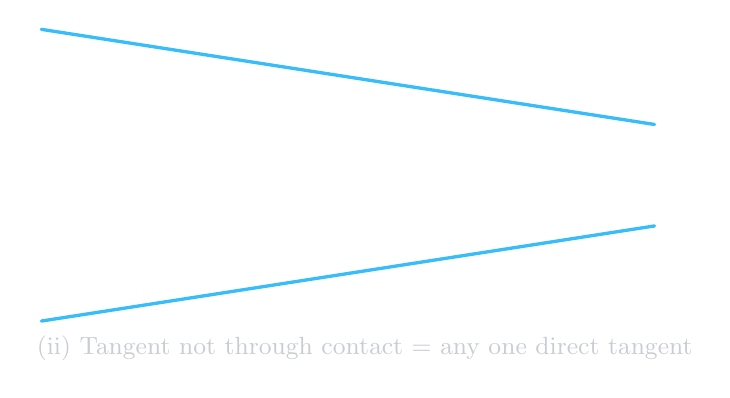
\begin{tikzpicture}[scale=1.02]
  \pgfmathsetmacro{\R}{1.44}
  \pgfmathsetmacro{\r}{1.04}
  \pgfmathsetmacro{\d}{2.48}
  \coordinate (O1) at (0,0);
  \coordinate (O2) at (\d,0);

  \draw[base] (O1) circle (\R);
  \draw[base] (O2) circle (\r);

  \pgfmathsetmacro{\nxE}{(\R-\r)/\d}
  \pgfmathsetmacro{\nyE}{sqrt(1-\nxE*\nxE)}
  \coordinate (P1t) at ({- \R*\nxE},{- \R*\nyE});
  \coordinate (P2t) at ({\d- \r*\nxE},{- \r*\nyE});
  \coordinate (P1b) at ({- \R*\nxE},{+ \R*\nyE});
  \coordinate (P2b) at ({\d- \r*\nxE},{+ \r*\nyE});

  \draw[new] ($(P1t)!-1.0!(P2t)$) -- ($(P1t)!2.0!(P2t)$);
  \draw[new] ($(P1b)!-1.0!(P2b)$) -- ($(P1b)!2.0!(P2b)$);

  \node[labm] at (1.25,-2.15) {(ii) Tangent not through contact = any one direct tangent};
\end{tikzpicture}
\end{StepDiagram}

\Step{4} The \textbf{two common tangents} (besides the contact one) are exactly these two direct tangents.
\begin{StepDiagram}
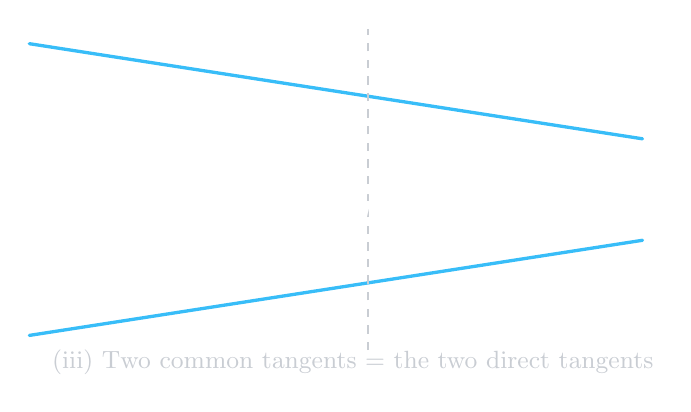
\begin{tikzpicture}[scale=1.02]
  \pgfmathsetmacro{\R}{1.44}
  \pgfmathsetmacro{\r}{1.04}
  \pgfmathsetmacro{\d}{2.48}
  \coordinate (O1) at (0,0);
  \coordinate (O2) at (\d,0);
  \coordinate (T)  at (\R,0);

  \draw[base] (O1) circle (\R);
  \draw[base] (O2) circle (\r);

  % two direct tangents
  \pgfmathsetmacro{\nxE}{(\R-\r)/\d}
  \pgfmathsetmacro{\nyE}{sqrt(1-\nxE*\nxE)}
  \coordinate (P1t) at ({- \R*\nxE},{- \R*\nyE});
  \coordinate (P2t) at ({\d- \r*\nxE},{- \r*\nyE});
  \coordinate (P1b) at ({- \R*\nxE},{+ \R*\nyE});
  \coordinate (P2b) at ({\d- \r*\nxE},{+ \r*\nyE});
  \draw[new] ($(P1t)!-1.0!(P2t)$) -- ($(P1t)!2.0!(P2t)$);
  \draw[new] ($(P1b)!-1.0!(P2b)$) -- ($(P1b)!2.0!(P2b)$);

  % contact tangent (shown faint)
  \draw[help] (\R,-2.0) -- (\R,2.0);

  \node[dot,label={[lab]below:$T$}] at (T) {};
  \node[labm] at (1.25,-2.15) {(iii) Two common tangents = the two direct tangents};
\end{tikzpicture}
\end{StepDiagram}

\end{QAPair}

% ============================================================
% Q10
\begin{QAPair}{Question 10}
\textcolor{gold}{\bfseries Question:} Construct two intersecting circles of radii $2.5$ cm and $3$ cm whose centres are $4.8$ cm apart. Draw two common tangents to the circles.
\tcblower
\textcolor{green}{\bfseries Construction:}\par

\Step{1} Draw $O_1O_2=4.8$ cm and circles of radii $3$ cm (at $O_1$) and $2.5$ cm (at $O_2$).
\begin{StepDiagram}
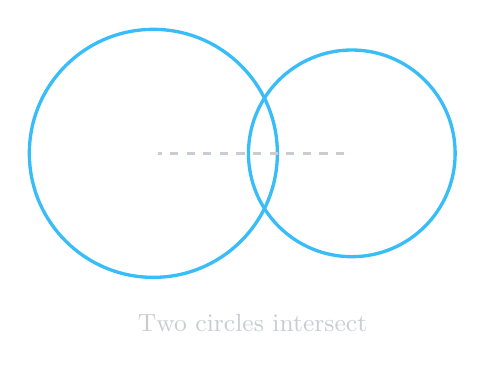
\begin{tikzpicture}[scale=1.05]
  \pgfmathsetmacro{\R}{1.50} % 3 scaled by 0.5
  \pgfmathsetmacro{\r}{1.25} % 2.5 scaled by 0.5
  \pgfmathsetmacro{\d}{2.40} % 4.8 scaled by 0.5
  \coordinate (O1) at (0,0);
  \coordinate (O2) at (\d,0);
  \draw[new] (O1) circle (\R);
  \draw[new] (O2) circle (\r);
  \draw[help] (O1)--(O2);
  \node[dot,label={[lab]below:$O_1$}] at (O1) {};
  \node[dot,label={[lab]below:$O_2$}] at (O2) {};
  \node[labm] at (1.2,-2.05) {Two circles intersect};
\end{tikzpicture}
\end{StepDiagram}

\Step{2} For direct tangents, draw auxiliary circle with centre $O_1$ and radius $(R-r)=0.5$ cm.
\begin{StepDiagram}
\begin{tikzpicture}[scale=1.05]
  \pgfmathsetmacro{\R}{1.50}
  \pgfmathsetmacro{\r}{1.25}
  \pgfmathsetmacro{\d}{2.40}
  \pgfmathsetmacro{\aux}{0.25} % 0.5 scaled by 0.5
  \coordinate (O1) at (0,0);
  \coordinate (O2) at (\d,0);
  \draw[base] (O1) circle (\R);
  \draw[base] (O2) circle (\r);
  \draw[new]  (O1) circle (\aux);
  \node[dot,label={[lab]below:$O_1$}] at (O1) {};
  \node[dot,label={[lab]below:$O_2$}] at (O2) {};
  \node[labm] at (1.2,-2.05) {Auxiliary circle of radius $R-r$};
\end{tikzpicture}
\end{StepDiagram}

\Step{3} From $O_2$, draw two tangents to the auxiliary circle.
\begin{StepDiagram}
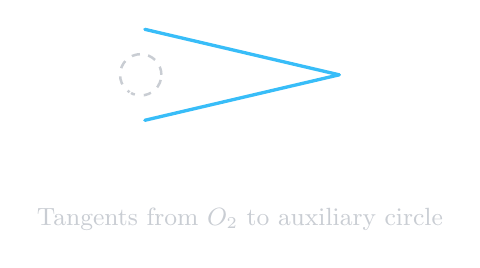
\begin{tikzpicture}[scale=1.05]
  \pgfmathsetmacro{\aux}{0.25}
  \coordinate (O1) at (0,0);
  \coordinate (O2) at (2.40,0);
  \draw[help] (O1) circle (\aux);
  \node[dot,label={[lab]below:$O_1$}] at (O1) {};
  \node[dot,label={[lab]below:$O_2$}] at (O2) {};
  \draw[new] (O2)--(0.05, 0.55);
  \draw[new] (O2)--(0.05,-0.55);
  \node[labm] at (1.2,-1.75) {Tangents from $O_2$ to auxiliary circle};
\end{tikzpicture}
\end{StepDiagram}

\Step{4} Draw parallels touching the smaller circle; these are the two common tangents.
\begin{StepDiagram}
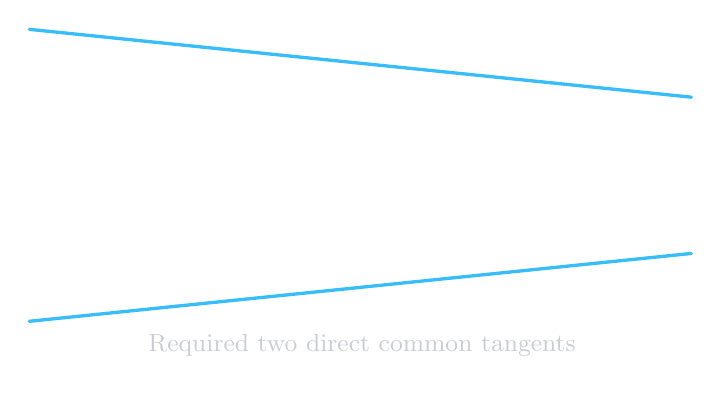
\begin{tikzpicture}[scale=1.05]
  \pgfmathsetmacro{\R}{1.50}
  \pgfmathsetmacro{\r}{1.25}
  \pgfmathsetmacro{\d}{2.40}
  \coordinate (O1) at (0,0);
  \coordinate (O2) at (\d,0);

  \draw[base] (O1) circle (\R);
  \draw[base] (O2) circle (\r);

  \pgfmathsetmacro{\nxE}{(\R-\r)/\d}
  \pgfmathsetmacro{\nyE}{sqrt(1-\nxE*\nxE)}
  \coordinate (P1t) at ({- \R*\nxE},{- \R*\nyE});
  \coordinate (P2t) at ({\d- \r*\nxE},{- \r*\nyE});
  \coordinate (P1b) at ({- \R*\nxE},{+ \R*\nyE});
  \coordinate (P2b) at ({\d- \r*\nxE},{+ \r*\nyE});

  \draw[new] ($(P1t)!-1.1!(P2t)$) -- ($(P1t)!2.2!(P2t)$);
  \draw[new] ($(P1b)!-1.1!(P2b)$) -- ($(P1b)!2.2!(P2b)$);

  \node[labm] at (1.2,-2.05) {Required two direct common tangents};
\end{tikzpicture}
\end{StepDiagram}

\end{QAPair}

% ============================================================
% Q11
\begin{QAPair}{Question 11}
\textcolor{gold}{\bfseries Question:} Two pulleys of radii $7$ in and $14$ in. Centres are $28$ in apart. Find approximate rope length.
\tcblower
\textcolor{green}{\bfseries Answer:}\par

\Step{1} Identify an \textbf{open belt}. Set $R=14$, $r=7$, $C=28$ (inches).
\begin{StepDiagram}
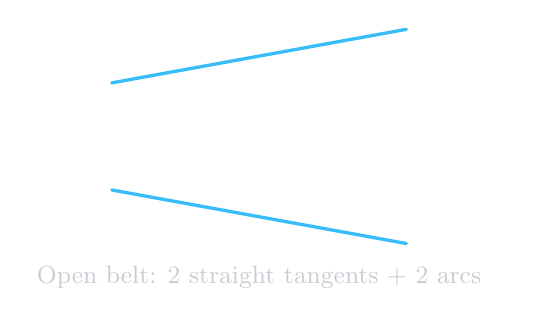
\begin{tikzpicture}[scale=0.85]
  \def\R{1.6}
  \def\r{0.8}
  \coordinate (O1) at (0,0);
  \coordinate (O2) at (4.2,0);
  \draw[base] (O1) circle (\r);
  \draw[base] (O2) circle (\R);
  \draw[new] (-0.1, \r) -- (4.3, \R);
  \draw[new] (-0.1,-\r) -- (4.3,-\R);
  \node[dot,label={[lab]below:$O_1$}] at (O1) {};
  \node[dot,label={[lab]below:$O_2$}] at (O2) {};
  \node[labm] at (2.1,-2.1) {Open belt: 2 straight tangents + 2 arcs};
\end{tikzpicture}
\end{StepDiagram}

\Step{2} Compute $\alpha=\sin^{-1}\!\left(\dfrac{R-r}{C}\right)=\sin^{-1}(0.25)$.
\EqDiagram{$\alpha=\sin^{-1}\!\left(\dfrac{14-7}{28}\right)=\sin^{-1}(0.25)\approx 0.25268\text{ rad}.$}

\Step{3} Use open-belt formula:
\[
L=2\sqrt{C^2-(R-r)^2}+\pi(R+r)+2\alpha(R-r).
\]
\EqDiagram{$L=2\sqrt{28^2-7^2}+\pi(21)+2\alpha\cdot 7$}

\Step{4} Substitute and approximate:
\[
L\approx 54.22+65.97+3.54\approx 123.73.
\]
\EqDiagram{$L\approx 123.7\text{ inches}\ (\approx 124\text{ inches}).$}

\[
\boxed{L\approx 123.7\ \text{inches}}
\]
\end{QAPair}

% ============================================================
% Q12
\begin{QAPair}{Question 12}
\textcolor{gold}{\bfseries Question:} A satellite is at altitude $7600$ km. Earth radius is $6400$ km.
How far is the satellite from city $P$ (tangent point)?
\tcblower
\textcolor{green}{\bfseries Answer:}\par

\Step{1} Draw the right triangle with $OP$ radius and $PA$ tangent.
\begin{StepDiagram}
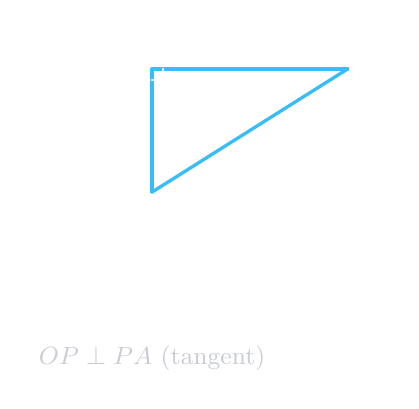
\begin{tikzpicture}[scale=0.92]
  \def\r{1.7}
  \coordinate (O) at (0,0);
  \coordinate (P) at (0,\r);
  \coordinate (A) at (2.7,1.7);
  \draw[base] (O) circle (\r);
  \node[dot,label={[lab]left:$O$}] at (O) {};
  \node[dot,label={[lab]above:$P$}] at (P) {};
  \node[dot,label={[lab]right:$A$}] at (A) {};
  \draw[new] (O)--(P);
  \draw[new] (O)--(A);
  \draw[new] (P)--(A);
  \draw[base] ($(P)+(0.15,0)$)--($(P)+(0.15,-0.15)$)--($(P)+(0,-0.15)$);
  \node[labm] at (0,-2.3) {$OP\perp PA$ (tangent)};
\end{tikzpicture}
\end{StepDiagram}

\Step{2} Compute distances from the centre:
\[
OP=6400,\quad OA=6400+7600=14000\ \text{km}.
\]
\EqDiagram{$OP=6400,\ \ OA=14000\text{ km}$}

\Step{3} Apply Pythagoras in right $\triangle OPA$:
\[
AP=\sqrt{OA^2-OP^2}.
\]
\EqDiagram{$AP=\sqrt{14000^2-6400^2}$}

\Step{4} Approximate:
\[
AP=\sqrt{155040000}\approx 12451.9\ \text{km}.
\]
\EqDiagram{$AP\approx 12452\text{ km}$}

\[
\boxed{AP\approx 12452\ \text{km}}
\]
\end{QAPair}

% ============================================================
% Q13
\begin{QAPair}{Question 13}
\textcolor{gold}{\bfseries Question:} Two cylindrical rods are bound with a strap. Each rod has diameter $12$ cm. How long is the strap?
\tcblower
\textcolor{green}{\bfseries Answer:}\par

\Step{1} Each rod radius $r=6$ cm. The strap is made of two straight parts and two semicircles.
\begin{StepDiagram}
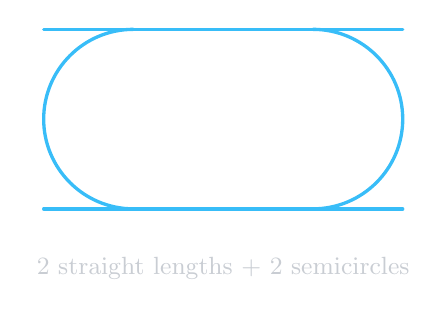
\begin{tikzpicture}[scale=0.95]
  \def\r{1.2}
  \coordinate (O1) at (0,0);
  \coordinate (O2) at (2.4,0);
  \draw[base] (O1) circle (\r);
  \draw[base] (O2) circle (\r);
  \draw[new] (-\r, \r) -- (2.4+\r, \r);
  \draw[new] (-\r,-\r) -- (2.4+\r,-\r);
  \draw[new] (0,\r) arc (90:270:\r);
  \draw[new] (2.4,\r) arc (90:-90:\r);
  \node[labm] at (1.2,-2.0) {2 straight lengths + 2 semicircles};
\end{tikzpicture}
\end{StepDiagram}

\Step{2} Total straight length: $2\times(2r)=4r=24$ cm.
\EqDiagram{Straight part: $4r=4(6)=24$ cm}

\Step{3} Curved part is a full circle of radius $r$: $2\pi r=12\pi$ cm.
\EqDiagram{Curved part: $2\pi r=2\pi(6)=12\pi$ cm}

\Step{4} Strap length:
\[
L=24+12\pi\approx 61.7\text{ cm}.
\]
\EqDiagram{$L=24+12\pi\approx 61.7$ cm}

\[
\boxed{L=24+12\pi\ \text{cm}\approx 61.7\ \text{cm}}
\]
\end{QAPair}

% ============================================================
% Q14
\begin{QAPair}{Question 14}
\textcolor{gold}{\bfseries Question:} A circular mirror has radius $20$ cm. It hangs by a wire from a hook.
The wire is $30$ cm long and is tangent to the mirror at two places. How far above the top of the mirror is the hook?
\tcblower
\textcolor{green}{\bfseries Answer:}\par

\Step{1} Tangents from the same external point are equal, so each wire segment to a tangency point is $15$ cm.
\begin{StepDiagram}
\begin{tikzpicture}[scale=0.95]
  \def\r{1.8}
  \coordinate (O) at (0,0);
  \coordinate (H) at (0,3.0);
  \draw[base] (O) circle (\r);
  \node[dot,label={[lab]below:$O$}] at (O) {};
  \node[dot,label={[lab]above:$H$}] at (H) {};
  \coordinate (T1) at ({\r*cos(60)},{\r*sin(60)});
  \coordinate (T2) at ({\r*cos(120)},{\r*sin(120)});
  \draw[new] (H)--(T1);
  \draw[new] (H)--(T2);
  \node[dot] at (T1) {}; \node[dot] at (T2) {};
  \node[lab, fill=pairbg, inner sep=1.2pt] at ($(H)!0.5!(T1)+(0.18,0.15)$) {$15$};
  \node[lab, fill=pairbg, inner sep=1.2pt] at ($(H)!0.5!(T2)+(-0.18,0.15)$) {$15$};
  \node[labm] at (0,-2.55) {Total wire $30$ cm $\Rightarrow$ each side $15$ cm};
\end{tikzpicture}
\end{StepDiagram}

\Step{2} Radius to tangency is perpendicular to tangent. So $\triangle OTH$ is right-angled with $OT=20$ cm and $HT=15$ cm.
\begin{StepDiagram}
\begin{tikzpicture}[scale=0.95]
  \def\r{1.8}
  \coordinate (O) at (0,0);
  \coordinate (H) at (0,3.0);
  \coordinate (T1) at ({\r*cos(60)},{\r*sin(60)});
  \draw[base] (O) circle (\r);
  \draw[new] (H)--(T1);
  \draw[new] (O)--(T1);
  \node[dot,label={[lab]below:$O$}] at (O) {};
  \node[dot,label={[lab]above:$H$}] at (H) {};
  \node[dot,label={[lab]right:$T$}] at (T1) {};
  \draw[base] ($(T1)+(-0.12,0)$) -- ($(T1)+(-0.12,-0.12)$) -- ($(T1)+(0,-0.12)$);
  \node[lab, fill=pairbg, inner sep=1.2pt] at ($(O)!0.55!(T1)+(0.18,0)$) {$20$};
  \node[lab, fill=pairbg, inner sep=1.2pt] at ($(H)!0.55!(T1)+(0.15,0.15)$) {$15$};
  \node[labm] at (0,-2.55) {$OT\perp HT$};
\end{tikzpicture}
\end{StepDiagram}

\Step{3} Use Pythagoras to find $OH$:
\[
OH=\sqrt{20^2+15^2}=25\text{ cm}.
\]
\EqDiagram{$OH=\sqrt{20^2+15^2}=\sqrt{625}=25$ cm}

\Step{4} The top of the mirror is $20$ cm above $O$, so height above top is $25-20=5$ cm.
\EqDiagram{Hook above top $=OH-20=25-20=5$ cm}

\[
\boxed{5\text{ cm}}
\]
\end{QAPair}

\end{document}
